\documentclass[aspectratio=169,10pt]{beamer}
\usetheme{default}
\usepackage{tikz}
\usepackage{array}
\usetikzlibrary{arrows.meta, positioning, fit, backgrounds}
\setbeamertemplate{navigation symbols}{}

% --- Fermilab-ish minimal look: white bg, blue sans titles, thin footer ------
\definecolor{fnalblue}{RGB}{0,84,159}
\definecolor{boxblue}{RGB}{40,90,160}
\definecolor{okgreen}{RGB}{0,130,60}
\setbeamercolor{frametitle}{fg=fnalblue}
\setbeamerfont{frametitle}{size=\Large,series=\bfseries}
\setbeamercolor{structure}{fg=fnalblue}
\setbeamertemplate{frametitle}{\vspace{0.4em}\insertframetitle\par}
\setbeamertemplate{footline}{%
  \hbox{\begin{beamercolorbox}[wd=\paperwidth,ht=2.5ex,dp=1.5ex,leftskip=1em,rightskip=1em]{}%
  \tiny\color{fnalblue}\insertdate\hfill Mu2e Genesis Meeting\hfill\insertframenumber%
  \end{beamercolorbox}}}
\setbeamercolor{itemize item}{fg=fnalblue}
\setbeamercolor{itemize subitem}{fg=fnalblue}

\newcolumntype{W}[1]{>{\raggedright\arraybackslash}p{#1}}

\title{\textcolor{fnalblue}{\textbf{Mu2e Genesis: Agentic Experiment Optimization}}}
\subtitle{\textcolor{fnalblue}{Workflow (i) --- activities and near-term plan}}
\author{Y.\ Oksuzian}
\institute{Argonne National Laboratory}
\date{8/10/2026}

\begin{document}

% ------------------------------------------------------------------ title
\begin{frame}[plain]
\vspace{2.2em}
\begin{center}
{\LARGE\bfseries\color{fnalblue} Mu2e Genesis: Agentic Experiment Optimization}\\[0.8em]
{\large\color{fnalblue} Workflow (i) --- activities and near-term plan}\\[3.5em]
{\large Y.\ Oksuzian}\\[0.3em]
{\large Argonne National Laboratory}\\[0.3em]
{\large Aug.\ 10, 2026}
\end{center}
\end{frame}

% ------------------------------------------------------- architecture loop
\begin{frame}{Agentic Experiment Optimization --- the loop}
\begin{center}
\textcolor{red}{\footnotesize Prompt-to-configuration: simulate, analyze, score, decide --- with a human gate.}
\end{center}
\vspace{-0.3em}
\begin{center}
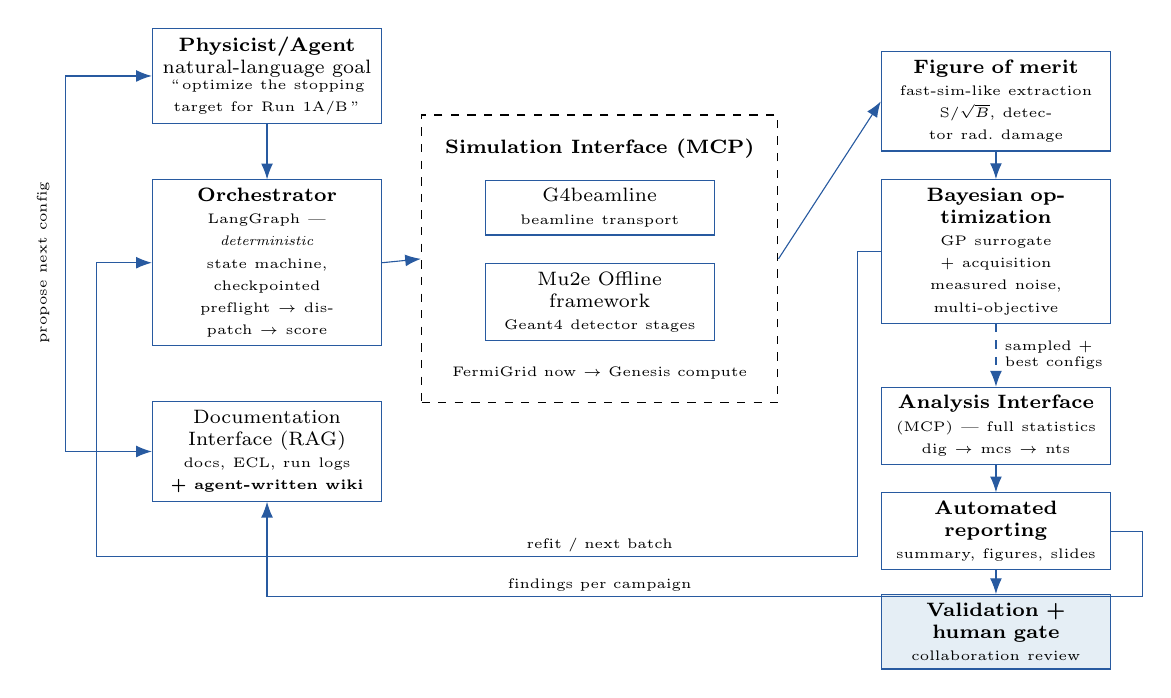
\begin{tikzpicture}[
  font=\scriptsize,
  box/.style={draw=boxblue, rectangle, align=center, inner sep=3pt, text width=27mm},
  grp/.style={draw=black, dashed, rectangle, inner sep=5pt},
  ar/.style={-{Latex[length=2mm]}, draw=boxblue}]

% --- left column: prompt -> agent -> docs
\node[box] (prompt) {\textbf{Physicist/Agent}\\natural-language goal\\{\tiny ``\,optimize the stopping\\target for Run 1A/B\,''}};
\node[box, below=7mm of prompt] (agent) {\textbf{Orchestrator}\\{\tiny LangGraph --- \emph{deterministic}}\\{\tiny state machine, checkpointed}\\{\tiny preflight $\rightarrow$ dispatch $\rightarrow$ score}};
\node[box, below=7mm of agent] (docs) {Documentation\\Interface (RAG)\\{\tiny docs, ECL, run logs}\\{\tiny \textbf{+ agent-written wiki}}};

% --- middle column: the Simulation Interface WRAPS both simulation engines
\node[box, right=13mm of agent, yshift=7mm] (g4bl) {G4beamline\\{\tiny beamline transport}};
\node[box, below=3.5mm of g4bl] (offline) {Mu2e Offline framework\\{\tiny Geant4 detector stages}};
\node[font=\scriptsize\bfseries, above=1.5mm of g4bl] (simtitle) {Simulation Interface (MCP)};
\node[font=\tiny, below=2mm of offline] (compute) {FermiGrid now $\rightarrow$ Genesis compute};
\begin{scope}[on background layer]
\node[grp, fit=(simtitle)(g4bl)(offline)(compute)] (simgrp) {};
\end{scope}

% --- right column: the FAST loop (FoM -> surrogate), then the gated
%     validation branch (full analysis chain on selected configs only)
\node[box, right=13mm of simgrp.east, yshift=20mm] (fom) {\textbf{Figure of merit}\\{\tiny fast-sim-like extraction}\\{\tiny S/$\sqrt{B}$, detector rad.\ damage}};
\node[box, below=3.5mm of fom] (gp) {\textbf{Bayesian optimization}\\{\tiny GP surrogate $+$ acquisition}\\{\tiny measured noise, multi-objective}};
\node[box, below=8mm of gp] (ana) {\textbf{Analysis Interface}\\{\tiny (MCP) --- full statistics}\\{\tiny dig $\rightarrow$ mcs $\rightarrow$ nts}};
\node[box, below=3.5mm of ana] (rep) {\textbf{Automated reporting}\\{\tiny summary, figures, slides}};
\node[box, below=3mm of rep, fill=fnalblue!10] (gate) {\textbf{Validation + human gate}\\{\tiny collaboration review}};

\coordinate (fby) at ([yshift=-7mm]docs.south);

\draw[ar] (prompt) -- (agent);
% Documentation feeds the PROPOSER, not the orchestrator: the state machine is
% deterministic and never queries a doc store (verified -- every wiki mention in
% graph/ is a code comment). The agent reads accumulated findings to propose the
% next configuration, and writes findings back. Routed left, clear of (agent).
\draw[{Latex[length=2mm]}-{Latex[length=2mm]}, draw=boxblue]
      (docs.west) -- ++(-11mm,0) |- (prompt.west);
\node[font=\tiny, rotate=90, anchor=south, align=center]
      at ([xshift=-11.8mm]agent.west) {propose next config};
\draw[ar] (agent.east) -- (simgrp.west);
\draw[ar] (simgrp.east) -- (fom.west);
\draw[ar] (fom) -- (gp);
\draw[ar, dashed] (gp) -- node[right, font=\tiny, align=left, inner sep=3pt] {sampled +\\best configs} (ana);
\draw[ar] (ana) -- (rep);
\draw[ar] (rep) -- (gate);
% SLOW loop (per campaign, knowledge): the batch report writes its findings BACK
% into the documentation store, so the next proposal is informed by what every
% previous batch learned. Implemented today as the wiki/ bundle (Karpathy
% LLM-wiki pattern, OKF v0.1) -- but written by the agent per session, not yet
% emitted automatically at drain. Outer lane, below the fast refit lane.
\coordinate (kby) at ([yshift=-12mm]docs.south);
\draw[ar] (rep.east) -- ++(4mm,0) |- (kby) -- (docs.south);
\node[anchor=south, inner sep=1.5pt] at (simgrp.south |- kby) {\tiny findings per campaign};
% feedback: surrogate -> agent, routed below the diagram
\draw[ar] (gp.west) -- ++(-0.3,0) |- (fby) -| ([xshift=-7mm]agent.west) |- (agent.west);
\node[anchor=south, inner sep=1.5pt] at (simgrp.south |- fby) {\tiny refit / next batch};
\end{tikzpicture}
\end{center}
\end{frame}

% ------------------------------------------------------------- activities 1
\begin{frame}{Activities and owners (1/2)}
\small
\textbf{Surrogate model optimization} \hfill \textcolor{fnalblue}{(Yuri)}
\begin{itemize}\small
  \item Bayesian optimization: GP surrogate $+$ multi-objective acquisition (sensitivity vs.\ detector radiation damage)
  \item Needed: multi-fidelity, transfer between scenarios
  \item Explore BO models for higher dimensionality: TuRBO, SAASBO, input warping
\end{itemize}
\vspace{0.8em}

\textbf{LangGraph orchestration} \hfill \textcolor{fnalblue}{(Yuri / Ray / Rob)}
\begin{itemize}\small
  \item One graph run $=$ one evaluation; checkpointed, resumable
  \item \textbf{Today: LangGraph $+$ Bayesian optimization, prompted and orchestrated by Claude} --- staying within Claude is a viable option
  \item Needed: expose through MCP, log traces
  \item Parameterize scenarios: beam intensity, solenoid field scale, arbitrary geometry configuration
\end{itemize}
\vspace{0.8em}

\textbf{Fast sim scoring, Run1A/B} \hfill \textcolor{fnalblue}{(Michael)}
\begin{itemize}\small
  \item Today's only scoring path: S/$\sqrt{B}$ $+$ radiation damage, no full reconstruction
  \item Needed: improve fast-sim performance; revisit Run 1B; agreement with full sim
  \item Explore other fast-sim options: beam optics, detector response
\end{itemize}
\end{frame}

% ------------------------------------------------------------- activities 2
\begin{frame}{Activities and owners (2/2)}
\small
\textbf{Full-sim validation (dig $\rightarrow$ mcs $\rightarrow$ nts)} \hfill \textcolor{fnalblue}{(Sophie / James)}
\begin{itemize}\scriptsize
  \item Full chain, full statistics: best configs $+$ every $\sim$10th point, run async
  \item Needed: calibration vs.\ the fast score; evidence bar and sign-off
\end{itemize}
\vspace{0.6em}

\textbf{Infrastructure --- MCP, LLM, computing} \hfill \textcolor{fnalblue}{(Ray / Rob)}
\begin{itemize}\scriptsize
  \item MCP servers, agent skills, model endpoints, compute
  \item FermiGrid now $\rightarrow$ Genesis compute; token $+$ CPU accounting
\end{itemize}
\vspace{0.6em}

\textbf{Documentation interface} \hfill \textcolor{fnalblue}{(Cole / Simon)}
\begin{itemize}\scriptsize
  \item Search over docs, ECL, run and configuration logs
  \item Needed: context for the optimizer --- which constraints are real
\end{itemize}
\vspace{0.6em}

\textbf{G4beamline} \hfill \textcolor{fnalblue}{(Yuri)}
\begin{itemize}\scriptsize
  \item MCP server prototype demonstrated --- \textbf{a proposal commitment} (App.\ 5)
  \item Needed: integrate into the existing workflow
\end{itemize}
\vspace{0.15em}

\textbf{Automated reporting} \hfill \textcolor{fnalblue}{(Rob / Yuri)}
\begin{itemize}\scriptsize
  \item Campaign drains $\rightarrow$ summary, figures, slides and write-up generated automatically
  \item Needed: regenerate on new rows; every number traceable to a leaderboard row
  \item \textbf{Write-back}: every campaign appends what it learned to the documentation interface --- an agent-maintained wiki (Karpathy pattern); today hand-written per session
\end{itemize}

\end{frame}

% ------------------------------------------------------------------ status
\begin{frame}{Status --- the loop runs end-to-end}
\vspace{-0.6em}
\begin{center}
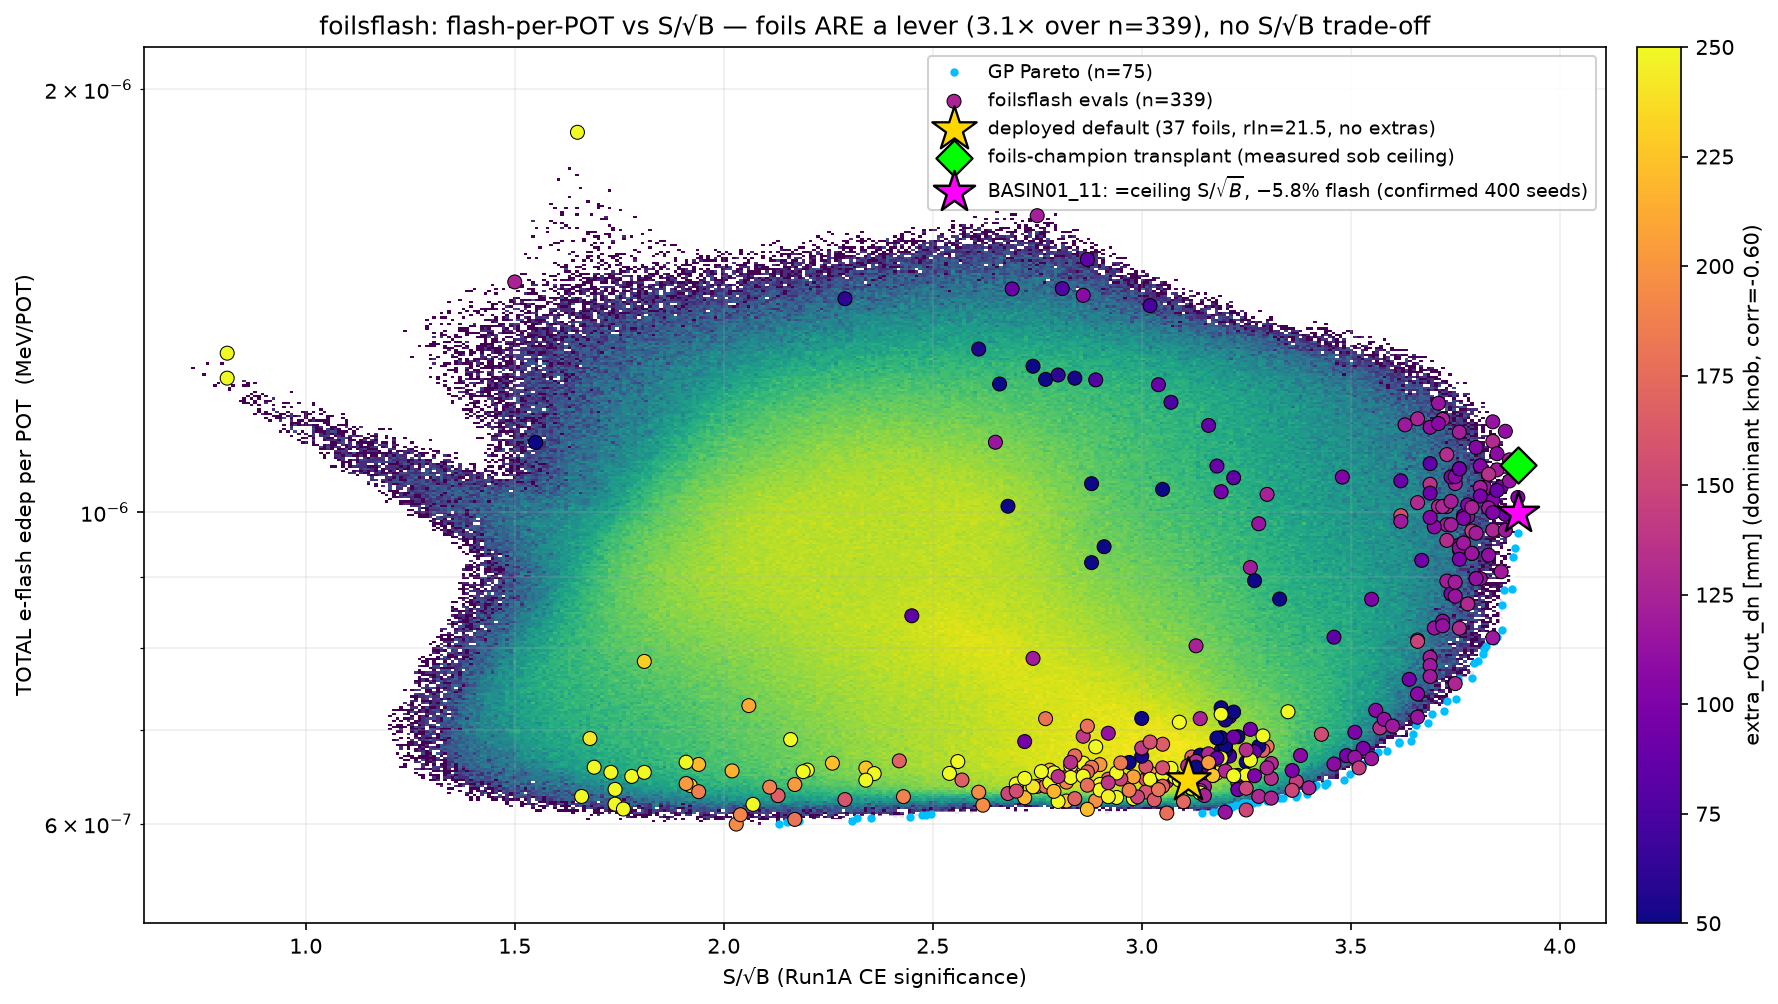
\includegraphics[width=0.60\textwidth]{foilsflash_perpot_cloud_nochamp.png}
\end{center}
\vspace{-0.2em}
\begin{columns}[T]
\begin{column}{0.55\textwidth}
\scriptsize
\begin{tabular}{@{}lcc@{}}
\hline
design & S/$\sqrt{B}$ & rad.\ damage \\
\hline
deployed default & 3.11 & 6.45$\times10^{-7}$ \\
\texttt{ff11R00\_07} (champion) & \textbf{3.31} & \textbf{6.26$\times10^{-7}$} \\
\texttt{ff14R01\_00} (exploit) & 3.84 & 8.14$\times10^{-7}$ \\
\texttt{BASIN01\_11} (confirmed) & \textbf{3.90} & 1.00$\times10^{-6}$ \\
\hline
\end{tabular}
\end{column}
\begin{column}{0.43\textwidth}
\scriptsize
\begin{itemize}\scriptsize
  \item \textbf{339} evaluations map a clean Pareto front
  \item Champion beats deployed on \textbf{both} axes: $+6\%$ S/$\sqrt{B}$ at $-3\%$ damage
  \item Best S/$\sqrt{B}$ \textbf{3.90 vs 3.11 deployed} $= \mathbf{+25\%}$, confirmed reproducible (400-seed)
\end{itemize}
\end{column}
\end{columns}
\end{frame}

% ------------------------------------------------------- target geometry
\begin{frame}{What the optimizer built --- the max-S/$\sqrt{B}$ target}
\begin{center}
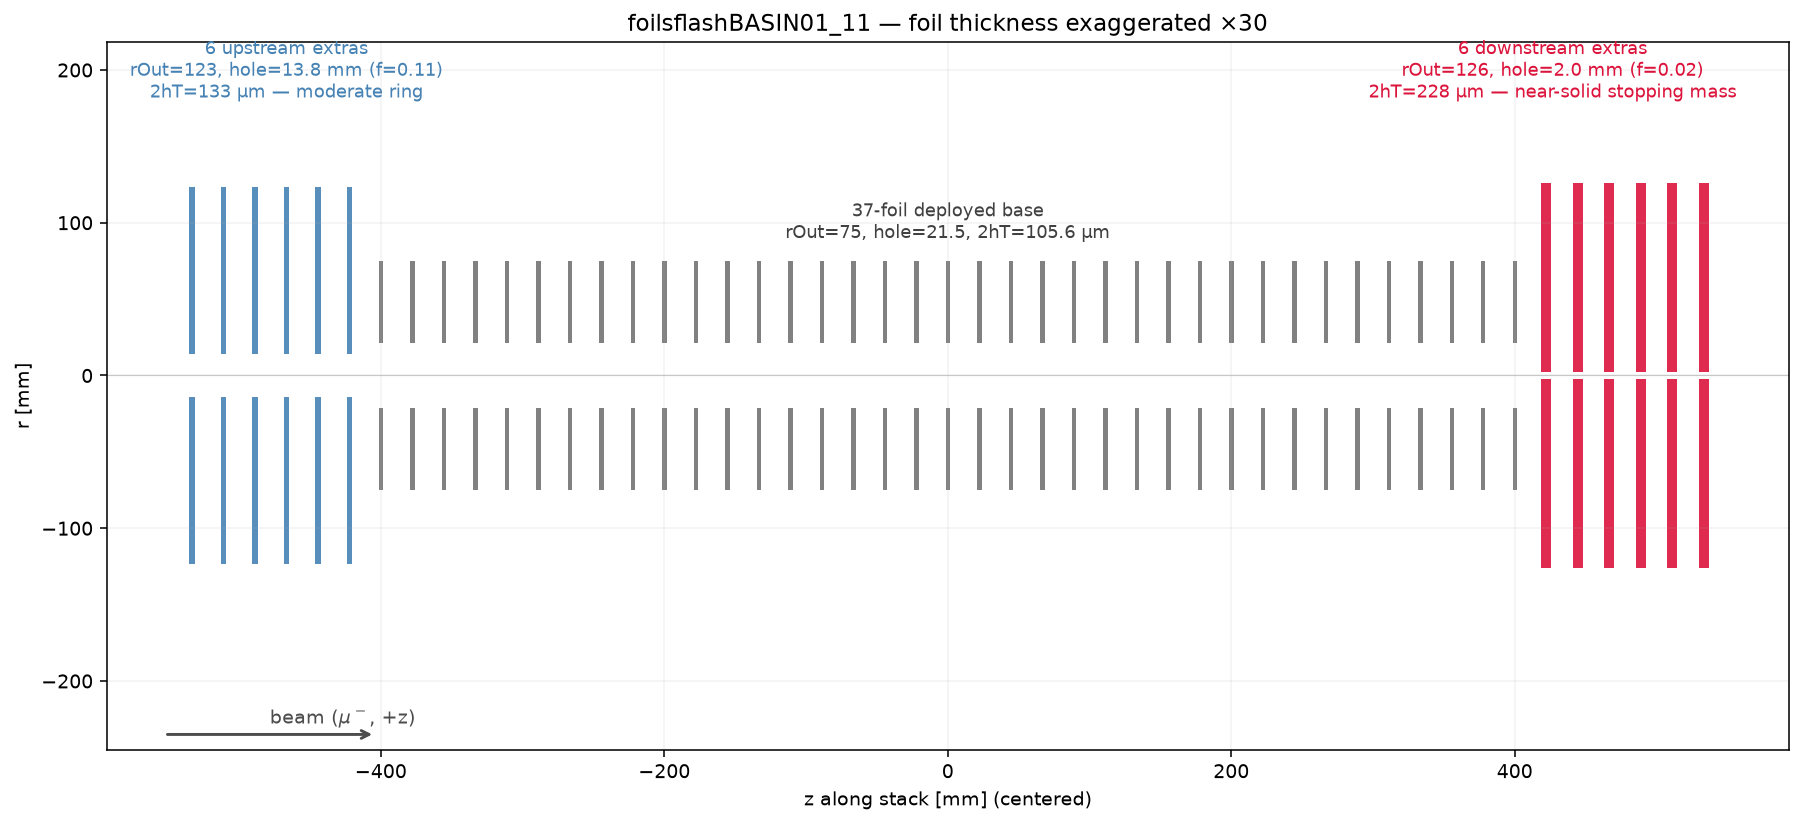
\includegraphics[width=0.92\textwidth]{foilsflash_bestsob_sketch.png}
\end{center}
\vspace{-0.2em}
\footnotesize
Two routes to high S/$\sqrt{B}$: a thin \textbf{off-beam ring}, or thin \textbf{in-beam}
material that degrades the beam to stop more muons. Here: 6 upstream extras (moderate ring)
$+$ 6 downstream (near-solid stopping mass) around the 37-foil deployed base.
\end{frame}

% ============================================ NEW LINE: profile-parameterized target
\begin{frame}{Since last time --- the whole target, not just the extras}
\vspace{-0.3em}
\begin{block}{}
\small
Second campaign line: throw away the hand-designed 37-foil base and let BO design
\textbf{all 49 foils} --- outer radius, thickness and central hole as smooth profiles,
plus the foil spacing. Everything stays inside the \textbf{deployed envelope}.
At the \emph{deployed damage budget} this gives \textbf{$+27\%$ S/$\sqrt{B}$}
(4.15 vs 3.26); unconstrained, the record is \textbf{4.41} $= +35\%$.
\end{block}
\vspace{-0.1em}
\begin{columns}[T]
\begin{column}{0.53\textwidth}
\vspace{-0.6em}
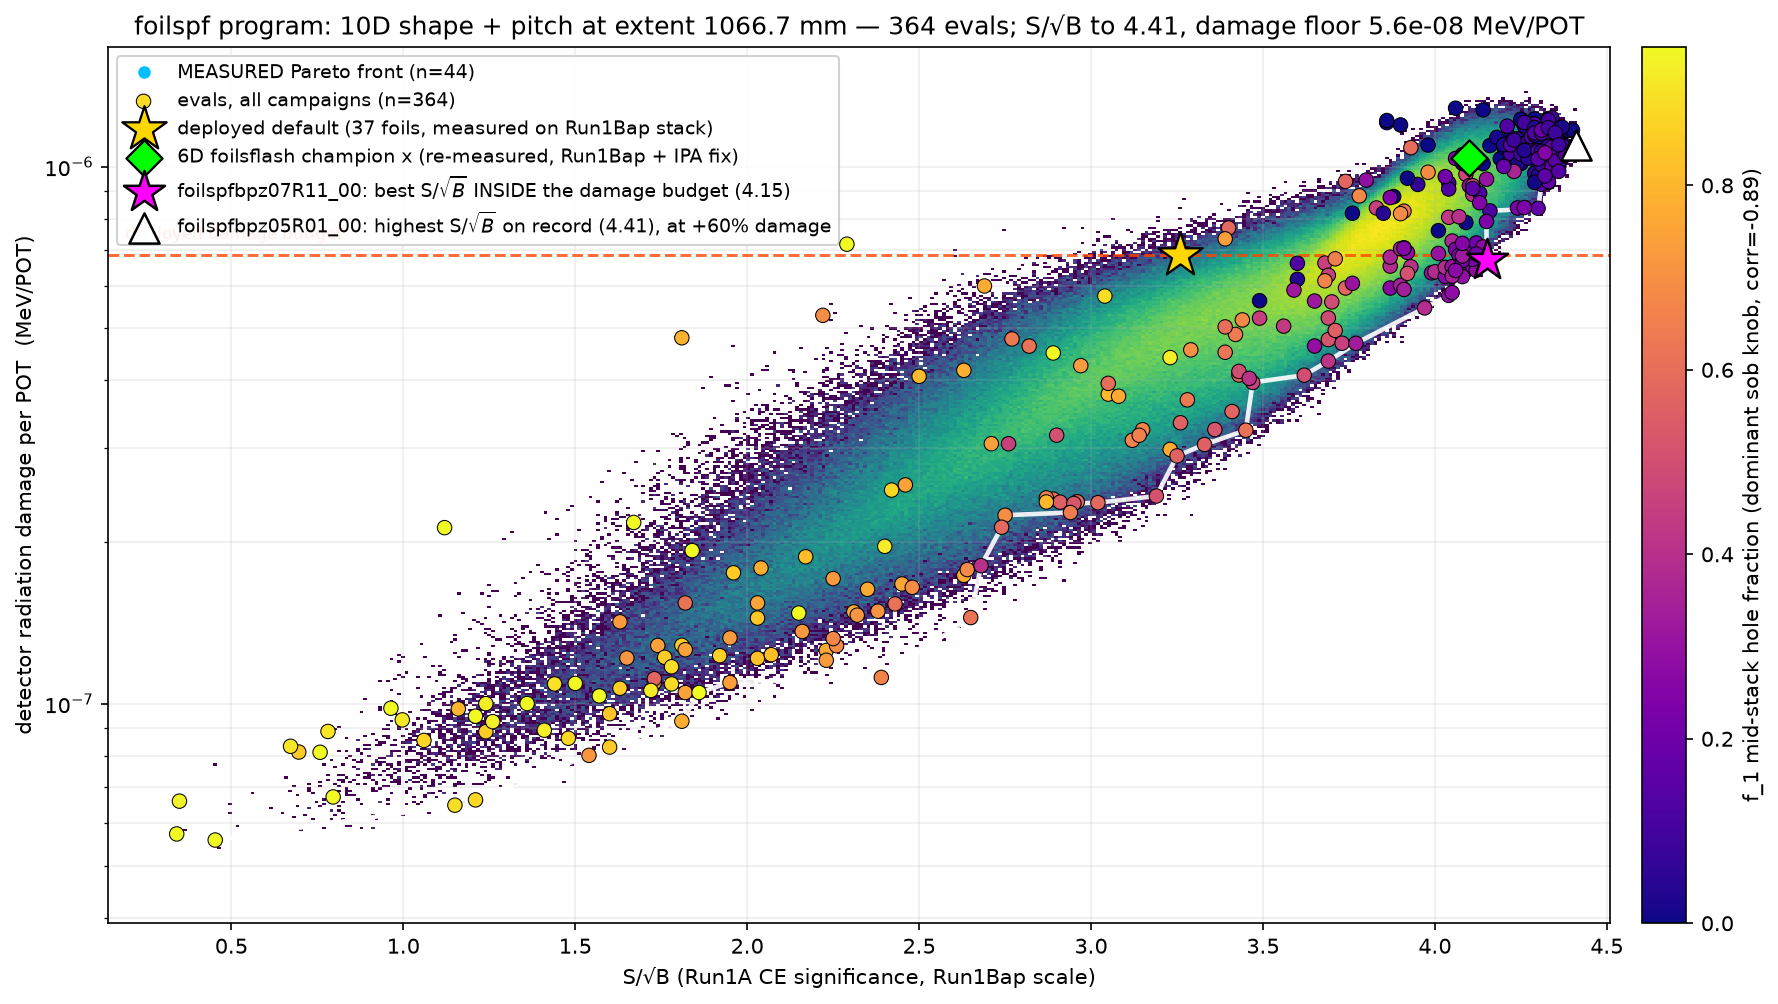
\includegraphics[width=\textwidth]{foilspfbpz_perpot_cloud_0810.png}
\end{column}
\begin{column}{0.45\textwidth}
\scriptsize
\begin{tabular}{@{}lcc@{}}
\hline
design & S/$\sqrt{B}$ & rad.\ damage \\
\hline
deployed default & 3.26 & 6.85$\times10^{-7}$ \\
\texttt{bpz07R11\_00} (deliverable) & \textbf{4.15} & \textbf{6.70$\times10^{-7}$} \\
\texttt{bpz05R01\_00} (record) & 4.41 & 1.10$\times10^{-6}$ \\
\hline
\end{tabular}
\vspace{0.5em}
\begin{itemize}\scriptsize
  \item \textbf{366} evaluations, twelve campaigns, \textbf{zero failures}
  \item The deliverable beats deployed on \textbf{both} axes: $+27\%$ S/$\sqrt{B}$
        at $-2\%$ damage. \textbf{63} designs do this
  \item \textbf{43} measured Pareto points; damage frontier spans \textbf{23$\times$}
  \item The old 4.00 plateau was an \textbf{acquisition artifact}: a picker
        aimed \emph{at} the damage budget beat it in 4 evaluations
\end{itemize}
\end{column}
\end{columns}
\end{frame}

% ------------------------------------------------- the record geometry + ceiling
\begin{frame}{The max-S/$\sqrt{B}$ design --- and how we knew to stop}
\begin{columns}[T]
\begin{column}{0.53\textwidth}
\vspace{-0.3em}
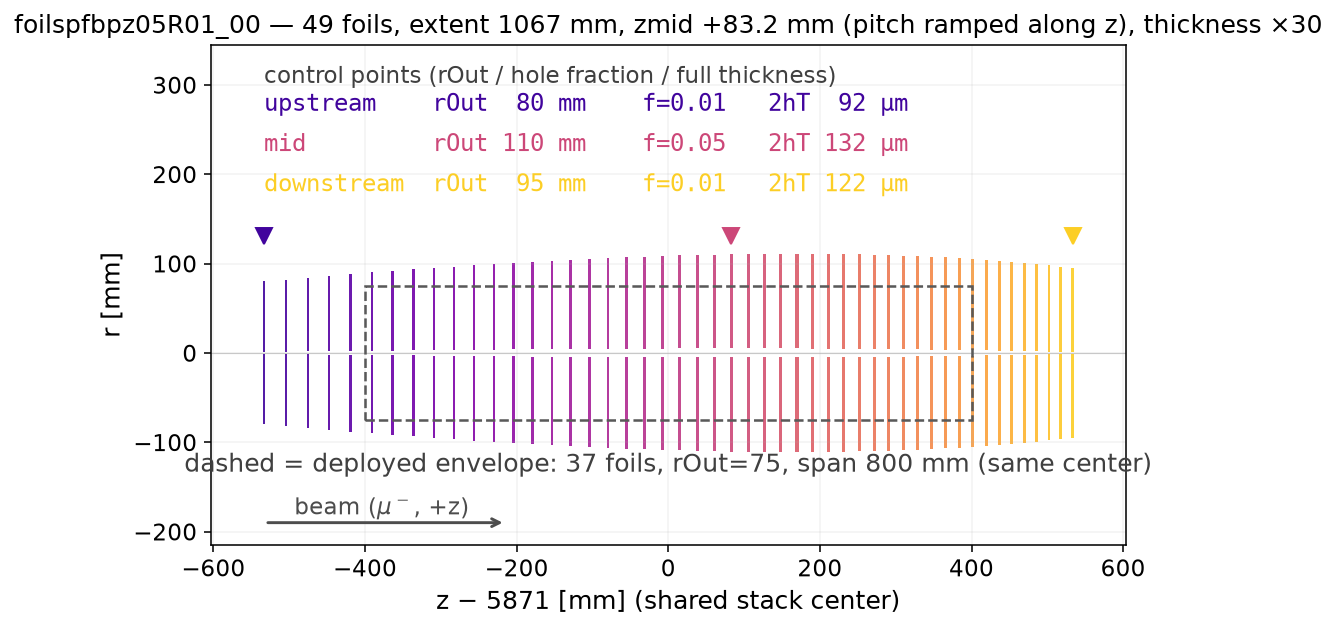
\includegraphics[width=\textwidth]{foilspfbpz05_bestsob_sketch.png}
\end{column}
\begin{column}{0.45\textwidth}
\footnotesize
\textbf{4.41 --- the unconstrained record.} A nearly \textbf{solid} stack (bore
$\le5$\,mm) as a gentle barrel, rOut $80\to110\to95$\,mm, foils \textbf{packed
downstream}. Nothing a human would have drawn.
\vspace{0.8em}

\textbf{Knowing when to stop is itself a result.} Acquisition ``saturation'' means the
\emph{frontier} stopped moving --- not that the space is mapped. Three dedicated
max-S/$\sqrt{B}$ rounds:
\vspace{0.3em}
\begin{center}
\normalsize 4.33 $\rightarrow$ 4.37 $\rightarrow$ \textbf{4.41} $\rightarrow$ 4.41\\
{\scriptsize two $\sim$5$\sigma$ steps, then flat}
\end{center}
\vspace{0.3em}

The third round: 40 evaluations, \textbf{nothing above 4.41} --- and the optimizer spent
a pick \textbf{re-measuring the record}, reproducing it exactly. Ridge mapped, line closed.
\end{column}
\end{columns}
\end{frame}

% ------------------------------------------- the deliverable: free improvement
\begin{frame}{The design we would actually deploy --- $+27\%$ for free}
\vspace{-0.2em}
\begin{columns}[T]
\begin{column}{0.55\textwidth}
\vspace{-0.4em}
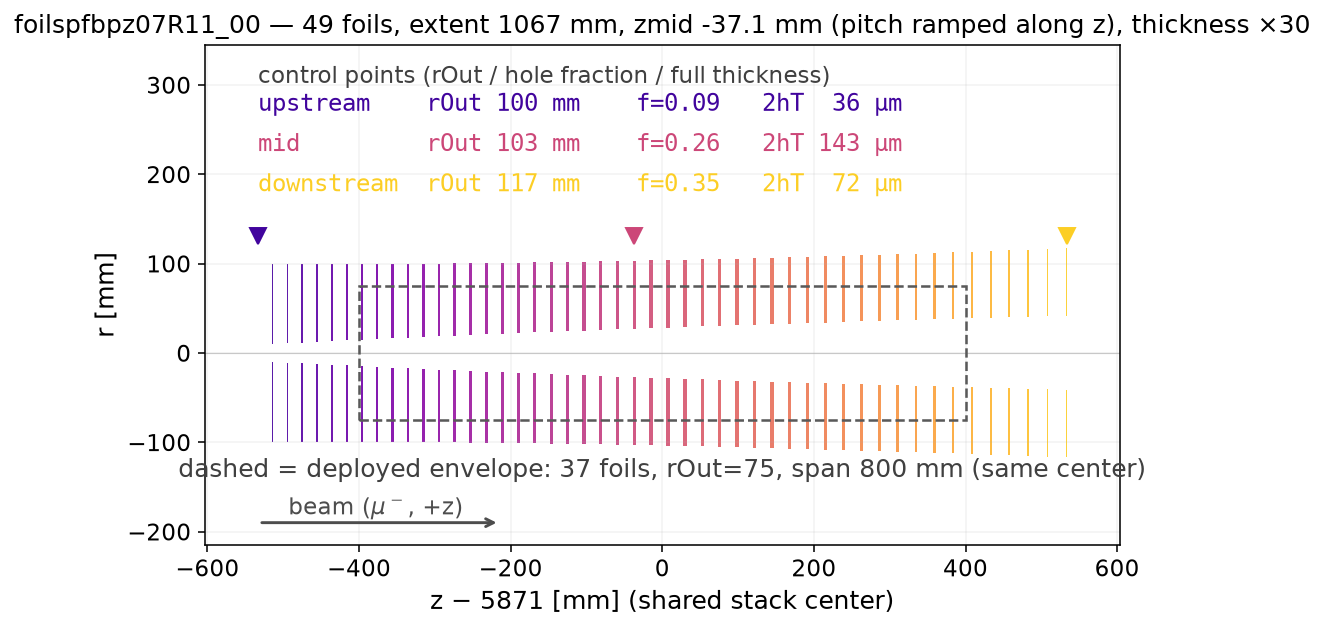
\includegraphics[width=\textwidth]{foilspf_budget_bpz07R11_00_sketch.png}
\end{column}
\begin{column}{0.43\textwidth}
\footnotesize
The record on the previous slide buys $+35\%$ by spending $+60\%$ more detector
damage. \textbf{This one is free.}
\vspace{0.3em}

\begin{center}
\scriptsize
\begin{tabular}{@{}lcc@{}}
\hline
 & S/$\sqrt{B}$ & rad.\ damage \\
\hline
deployed default & 3.26 & 6.85$\times10^{-7}$ \\
\texttt{bpz07R11\_00} & \textbf{4.15} & \textbf{6.70$\times10^{-7}$} \\
\emph{difference} & \textbf{$+27\%$} & \textbf{$-2\%$} \\
\hline
\end{tabular}
\end{center}
\vspace{0.2em}

\textbf{Better on \emph{both} axes} than the target now in the beam ---
\textbf{63} of 366 designs are, and this is the best of them.
\vspace{0.6em}

\textbf{The shape:} a near-cylindrical stack, rOut $100\to103\to117$\,mm, with a
\textbf{gradually opening bore} ($f = 0.09\to0.26\to0.35$) and the mass concentrated
mid-stack (36/143/72\,µm). Mass off-axis where it stops muons, beam core through
the hole instead of into the detector.
\end{column}
\end{columns}
\end{frame}

% --------------------------------------------------------------- milestones §4
\begin{frame}{Phase I milestones --- where Workflow (i) stands}
\small
9 months from \textbf{1 Aug 2026}; go/no-go at month 6 (Jan 2027). \textbf{We are in month 1.}
\vspace{0.6em}
\begin{center}
\scriptsize
\begin{tabular}{@{}llll@{}}
\hline
\textbf{window} & \textbf{dates} & \textbf{milestone (Workflow (i) parts)} & \textbf{status} \\
\hline
Months 1--2 & Aug--Sep 26 & Deploy interfaces: Simulation, Analysis, Documentation & \textcolor{red}{pending} \\
            &             & End-to-end agentic chain: sim $\rightarrow$ analysis $\rightarrow$ FoM & \textcolor{okgreen}{\textbf{done}} \\[0.3em]
Months 3--4 & Oct--Nov 26 & Exercise optimization on campaigns; collect metrics & \textcolor{okgreen}{\textbf{ahead}} \\[0.3em]
Months 5--6 & Dec--Jan 27 & Compile go/no-go results; \textbf{all traces logged} & \textcolor{red}{traces = gap} \\[0.3em]
Months 7--9 & Feb--Apr 27 & Harden interfaces; package artifacts for Genesis & --- \\
\hline
\end{tabular}
\end{center}
\vspace{0.6em}
\begin{itemize}\small
  \item One month in: the \textbf{science milestone of months 3--4 is already met}; interfaces are the open item
  \item Proposal \S4 anticipates this: \emph{``initial workflow prototyping can use simplified interfaces while production versions are improved''}
\end{itemize}
\end{frame}

% --------------------------------------------------------------- gate metrics
\begin{frame}{Decision gate metrics --- Workflow (i), proposal \S6}
\footnotesize
\textbf{(a)} \emph{``Closed-loop sim--analysis--optimization (agent-orchestrated search with Bayesian
optimization for local sampling) demonstrated on $\ge$\,2 distinct external-constraint scenarios
(e.g.\ half beam intensity, 10\% reduced fields), each initiated by a natural-language prompt and
completed within one week (vs.\ months for the manual baseline), with full traces logged''}
\begin{itemize}\footnotesize
  \item[$\rightarrow$] \textbf{Started.} Prompt $\rightarrow$ new mode $+$ 20 evaluations, saturation confirmed by a second campaign --- a scenario answers \textbf{within a day} (bar: one week)
  \item[$\rightarrow$] Remaining: the two \textbf{external-constraint} scenarios --- reduced / absent DS field, half beam intensity --- and \textbf{formal trace logging}
\end{itemize}
\vspace{0.7em}

\textbf{(b)} \emph{``for a Run-1a scenario (no full cosmic ray veto coverage), starting from the
collaboration's existing manually-optimized baseline, agent-produced configuration achieves improved
$R_{\mu e}$ sensitivity, with improvements documented for collaboration review''}
\begin{itemize}\footnotesize
  \item[$\rightarrow$] \textcolor{okgreen}{\textbf{Demonstrated twice, independently}} --- both lines beat the manually-optimized baseline on \textbf{both} axes:
  \begin{itemize}\scriptsize
    \item extras-only line: $+6\%$ S/$\sqrt{B}$ at $-3\%$ damage; $+25\%$ at the confirmed ceiling
    \item \textbf{full-target profile line (new)}: $\mathbf{+27\%}$ S/$\sqrt{B}$ at $\mathbf{-2\%}$ damage, \textbf{63} such designs; $+35\%$ at the mapped ceiling
  \end{itemize}
  \item[$\rightarrow$] To finish: \textbf{prove it with full sims} (dig $\rightarrow$ mcs $\rightarrow$ nts) on the best configs; scope by background regime; document for review
\end{itemize}
\end{frame}


% =========================================================== BACKUP
\begin{frame}[plain]
\vspace{2.5em}
\begin{center}
{\Large\bfseries\color{fnalblue} Backup}
\end{center}
\end{frame}

% ============================ top-5 DEPLOYABLE designs, one per slide
\begin{frame}{The five best \emph{deployable} designs}
\footnotesize
Every design here is measured \textbf{at or below the deployed damage budget} ---
unlike the unconstrained record and the five that follow, these could go in the
beam. All five come from \texttt{bpz07}, the one campaign whose acquisition was
aimed \emph{at} the constraint.
\vspace{0.5em}
\begin{center}
\scriptsize
\begin{tabular}{@{}clcccl@{}}
\hline
\# & design & S/$\sqrt{B}$ & vs deployed & damage & shape \\
\hline
1 & \texttt{bpz07R11\_00} & \textbf{4.15} & $\mathbf{+27\%}$ & $-2\%$ & near-cylindrical, gradually opening bore \\
2 & \texttt{bpz07R05\_00} & 4.12 & $+26\%$ & $-6\%$ & narrow throat, wide body, packed downstream \\
3 & \texttt{bpz07R00\_01} & 4.11 & $+26\%$ & $-6\%$ & narrowest throat, uniform pitch \\
4 & \texttt{bpz07R09\_00} & 4.11 & $+26\%$ & $-2\%$ & widest downstream bore ($f=0.52$) \\
5 & \texttt{bpz07R08\_00} & 4.08 & $+25\%$ & $-9\%$ & solid upstream face; cheapest damage \\
\hline
\end{tabular}
\end{center}
\vspace{0.5em}
\begin{itemize}\footnotesize
  \item The previous best deployable design was \textbf{4.00}, and three campaigns
        had failed to beat it --- \textbf{all five of these do}
  \item A \textbf{spread of shapes}, not one recipe: upstream rOut 41--100\,mm,
        bore fractions 0.02--0.33, pitch uniform to strongly ramped
  \item Every one of the five has \textbf{damage to spare} ($-2$ to $-9\%$), so
        none is scraping the constraint to get its score
\end{itemize}
\end{frame}

\begin{frame}{Deployable \#1 --- \texttt{bpz07R11\_00}, S/$\sqrt{B}$ = 4.15}
\begin{center}
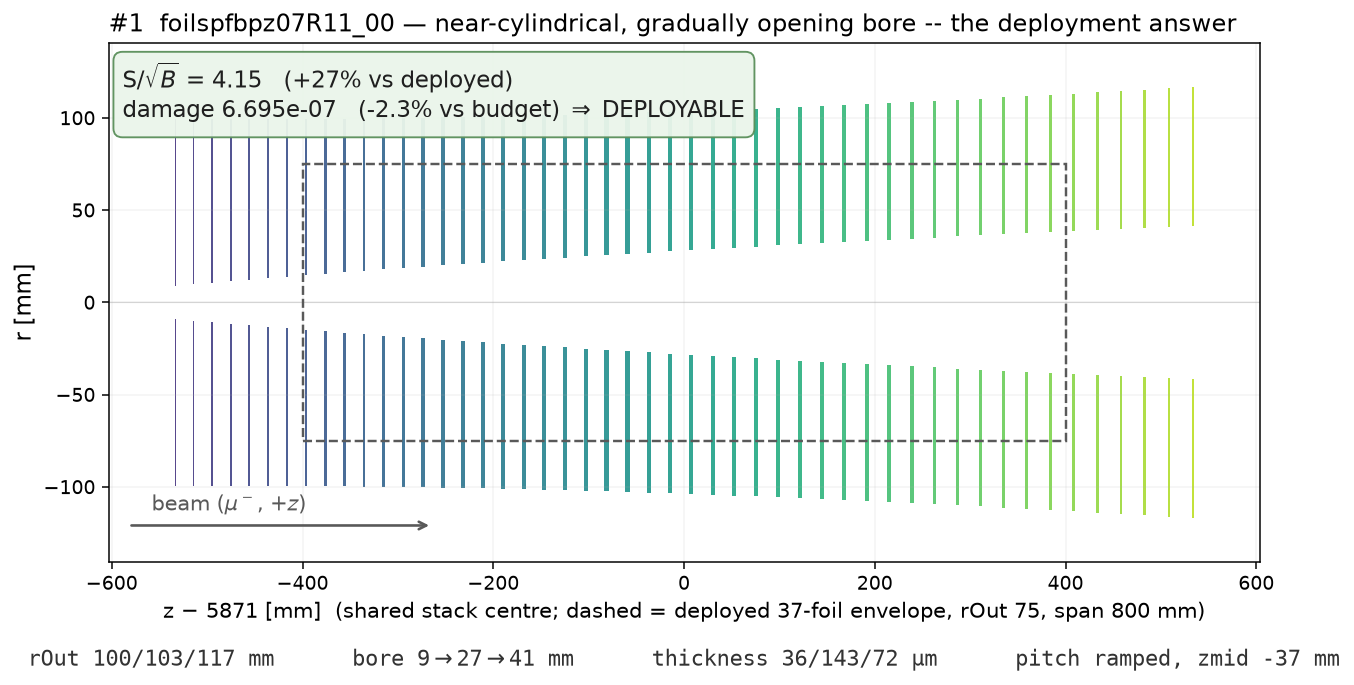
\includegraphics[width=0.95\textwidth]{foilspf_budget_top1_foilspfbpz07R11_00.png}
\end{center}
\end{frame}

\begin{frame}{Deployable \#2 --- \texttt{bpz07R05\_00}, S/$\sqrt{B}$ = 4.12}
\begin{center}
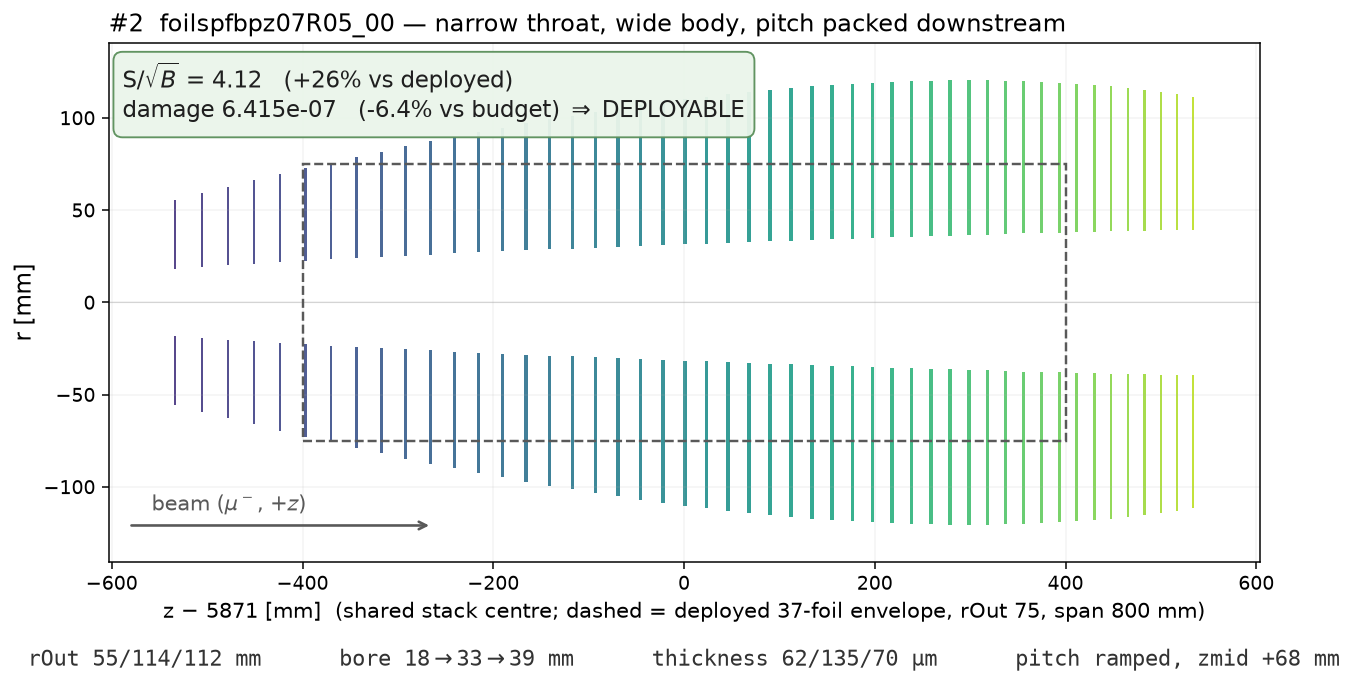
\includegraphics[width=0.95\textwidth]{foilspf_budget_top2_foilspfbpz07R05_00.png}
\end{center}
\end{frame}

\begin{frame}{Deployable \#3 --- \texttt{bpz07R00\_01}, S/$\sqrt{B}$ = 4.11}
\begin{center}
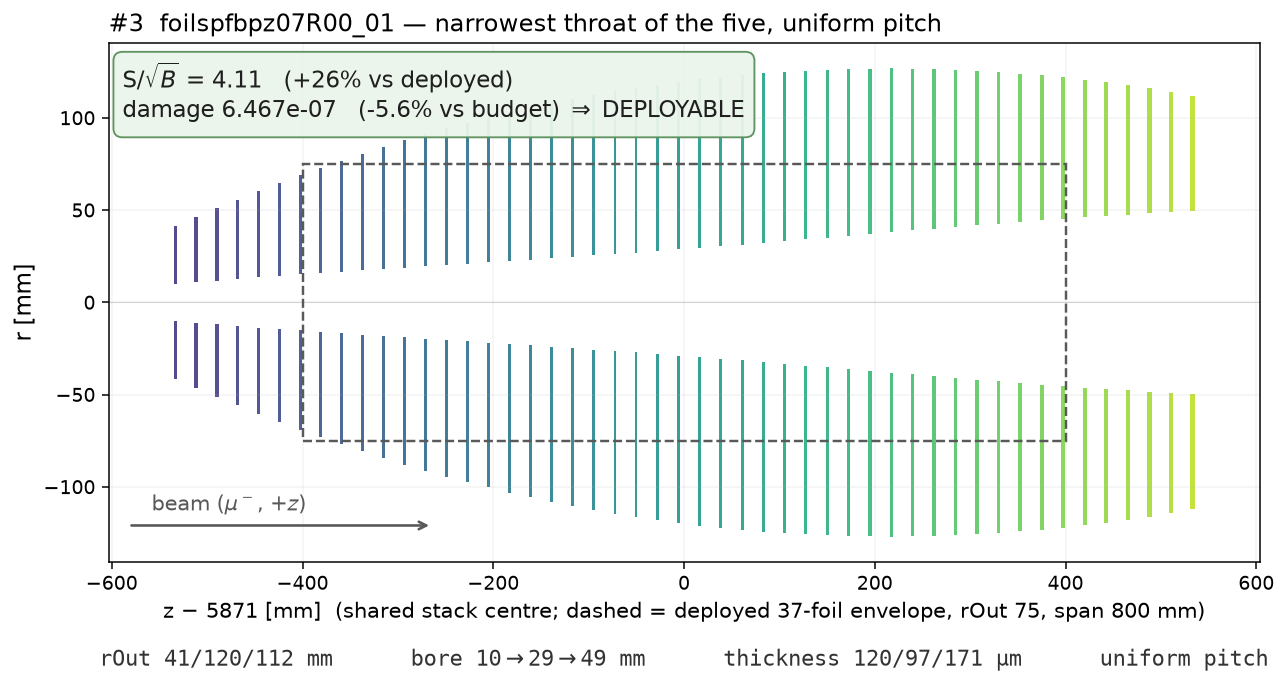
\includegraphics[width=0.95\textwidth]{foilspf_budget_top3_foilspfbpz07R00_01.png}
\end{center}
\end{frame}

\begin{frame}{Deployable \#4 --- \texttt{bpz07R09\_00}, S/$\sqrt{B}$ = 4.11}
\begin{center}
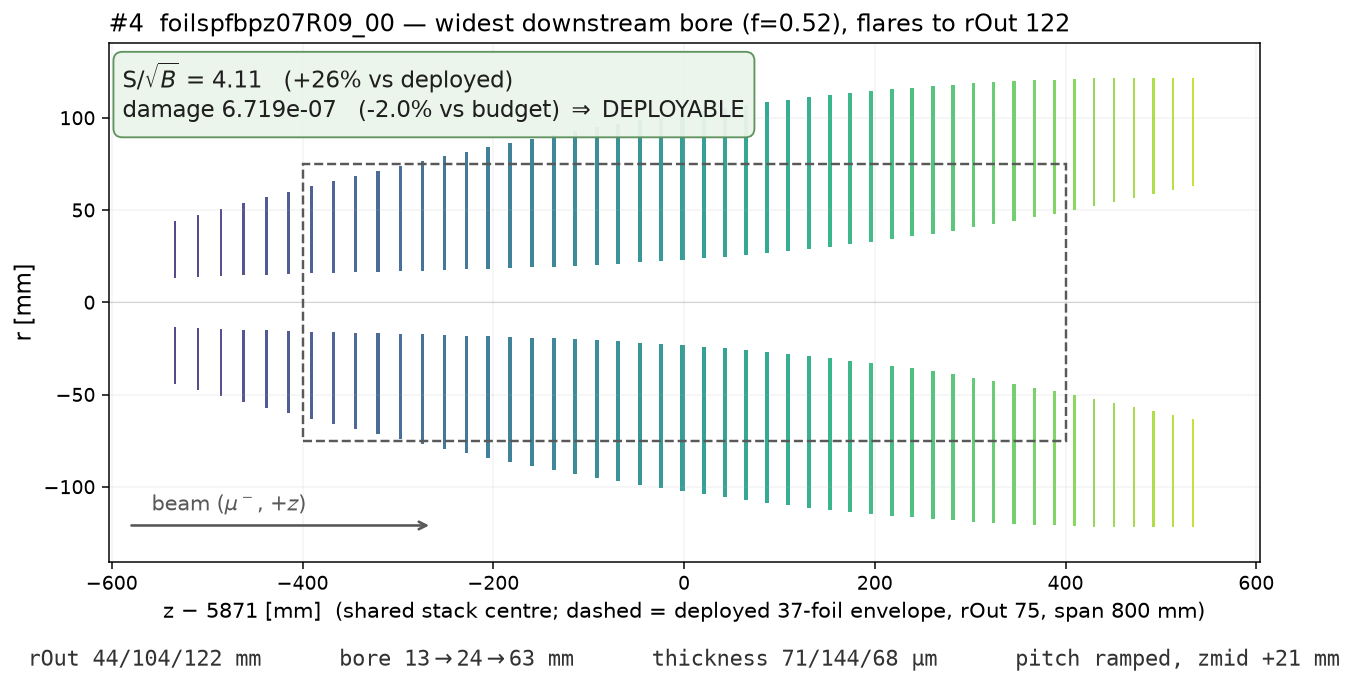
\includegraphics[width=0.95\textwidth]{foilspf_budget_top4_foilspfbpz07R09_00.png}
\end{center}
\end{frame}

\begin{frame}{Deployable \#5 --- \texttt{bpz07R08\_00}, S/$\sqrt{B}$ = 4.08}
\begin{center}
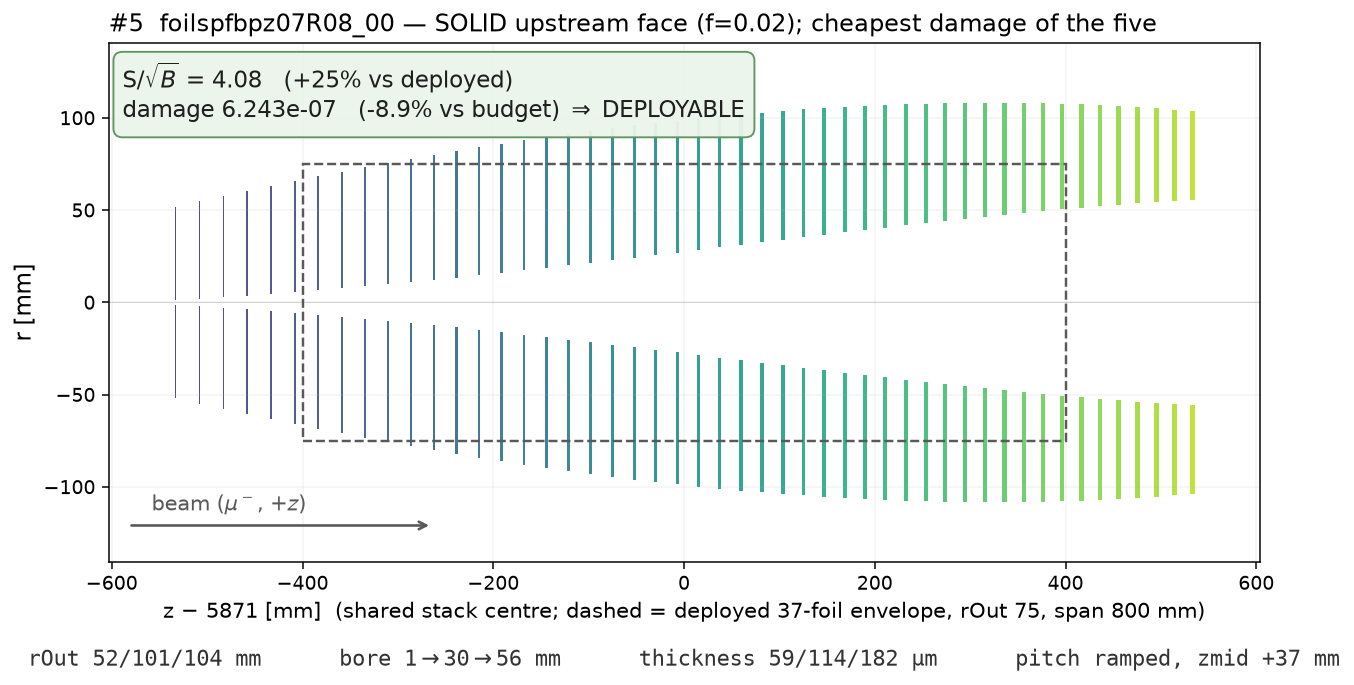
\includegraphics[width=0.95\textwidth]{foilspf_budget_top5_foilspfbpz07R08_00.png}
\end{center}
\end{frame}

% ------------------------------------------- top-5 designs, one per slide
\begin{frame}{The five best designs OVER budget --- one ridge top, five shapes}
\footnotesize
The optimizer's five best distinct targets score \textbf{4.38--4.41} --- a spread of
0.03, i.e.\ $\sim$5$\sigma$ total --- yet look nothing alike. That degeneracy is the
evidence the ceiling is mapped: many roads reach the same height, and none goes higher.
\vspace{0.5em}
\begin{center}
\scriptsize
\begin{tabular}{@{}clccl@{}}
\hline
\# & design & S/$\sqrt{B}$ & damage & shape \\
\hline
1 & \texttt{bpz05R01\_00} & \textbf{4.41} & $+60\%$ & near-solid barrel, pitch packed downstream \\
2 & \texttt{bpz06R04\_00} & 4.40 & $+71\%$ & solid, pitch at the box edge \\
3 & \texttt{bpz05R04\_03} & 4.38 & $+60\%$ & small bore, very thick downstream foils \\
4 & \texttt{bpz05R08\_00} & 4.38 & $+56\%$ & modest bore, \emph{uniform} pitch \\
5 & \texttt{bpz06R11\_00} & 4.38 & $+53\%$ & wide-mouth funnel bore, uniform pitch \\
\hline
\end{tabular}
\end{center}
\vspace{0.5em}
\begin{itemize}\footnotesize
  \item \textbf{Three of the five were measured twice} (different campaigns, independent
        seeds) and reproduced --- the ridge top is real, not a set of lucky draws
  \item Two opposite hole strategies --- \textbf{shut the bore} (\#1--3) vs.\ \textbf{open a
        funnel} (\#5) --- reach the same score
  \item All five are \textbf{damage-unconstrained}; the deployment answer is
        \texttt{bpz07R11\_00} at \textbf{4.15} \emph{inside} the deployed budget
\end{itemize}
\end{frame}

\begin{frame}{\#1 --- \texttt{bpz05R01\_00}, S/$\sqrt{B}$ = 4.41 (the record)}
\begin{center}
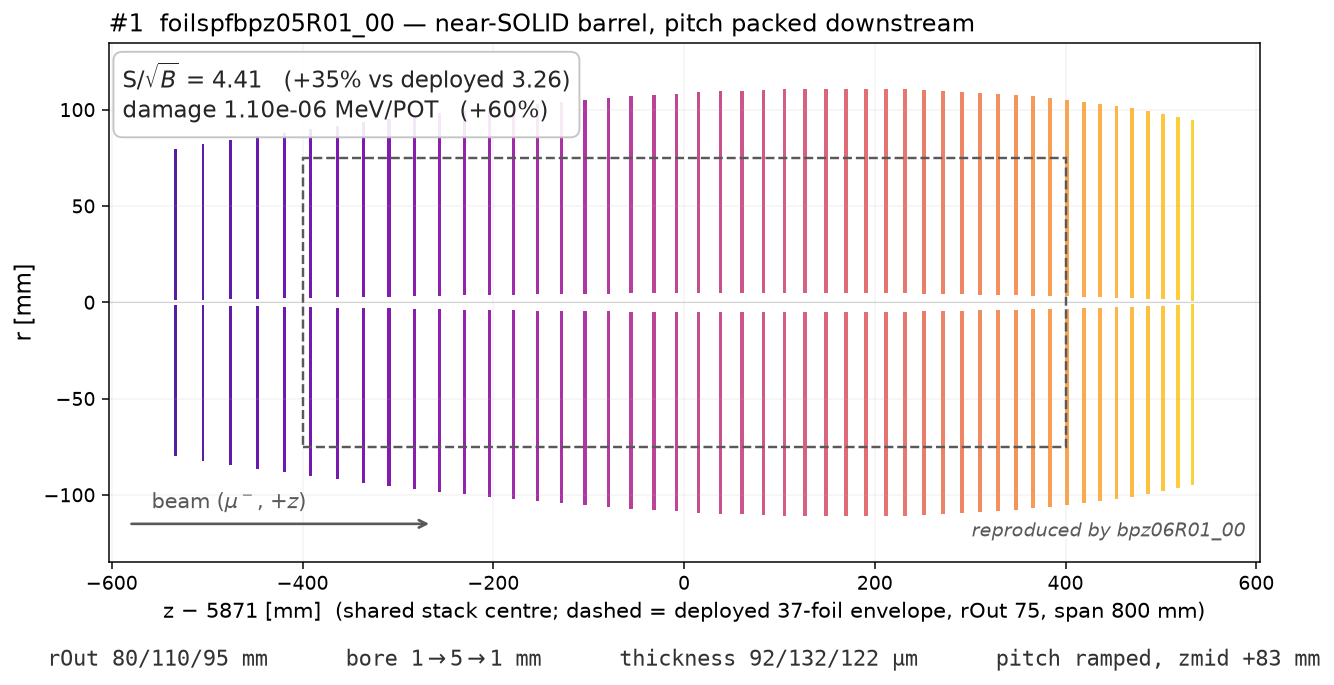
\includegraphics[width=0.95\textwidth]{foilspf_top1_foilspfbpz05R01_00.png}
\end{center}
\end{frame}

\begin{frame}{\#2 --- \texttt{bpz06R04\_00}, S/$\sqrt{B}$ = 4.40}
\begin{center}
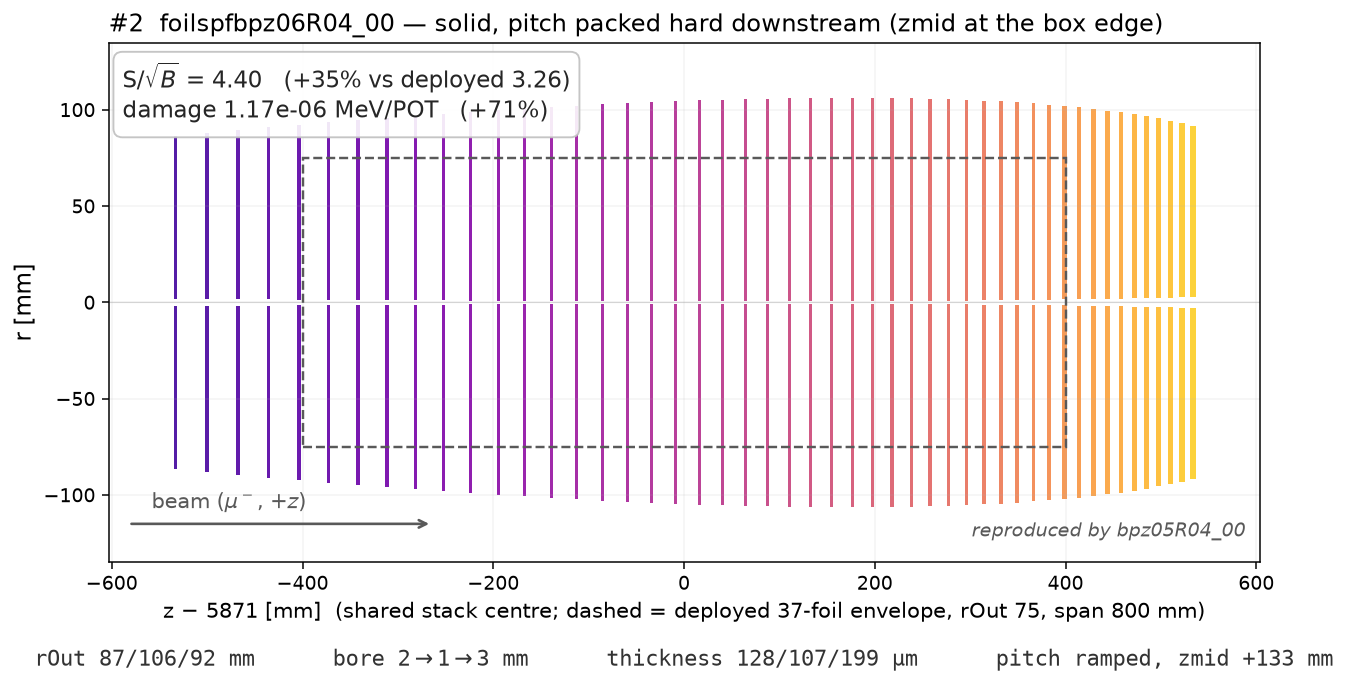
\includegraphics[width=0.95\textwidth]{foilspf_top2_foilspfbpz06R04_00.png}
\end{center}
\end{frame}

\begin{frame}{\#3 --- \texttt{bpz05R04\_03}, S/$\sqrt{B}$ = 4.38}
\begin{center}
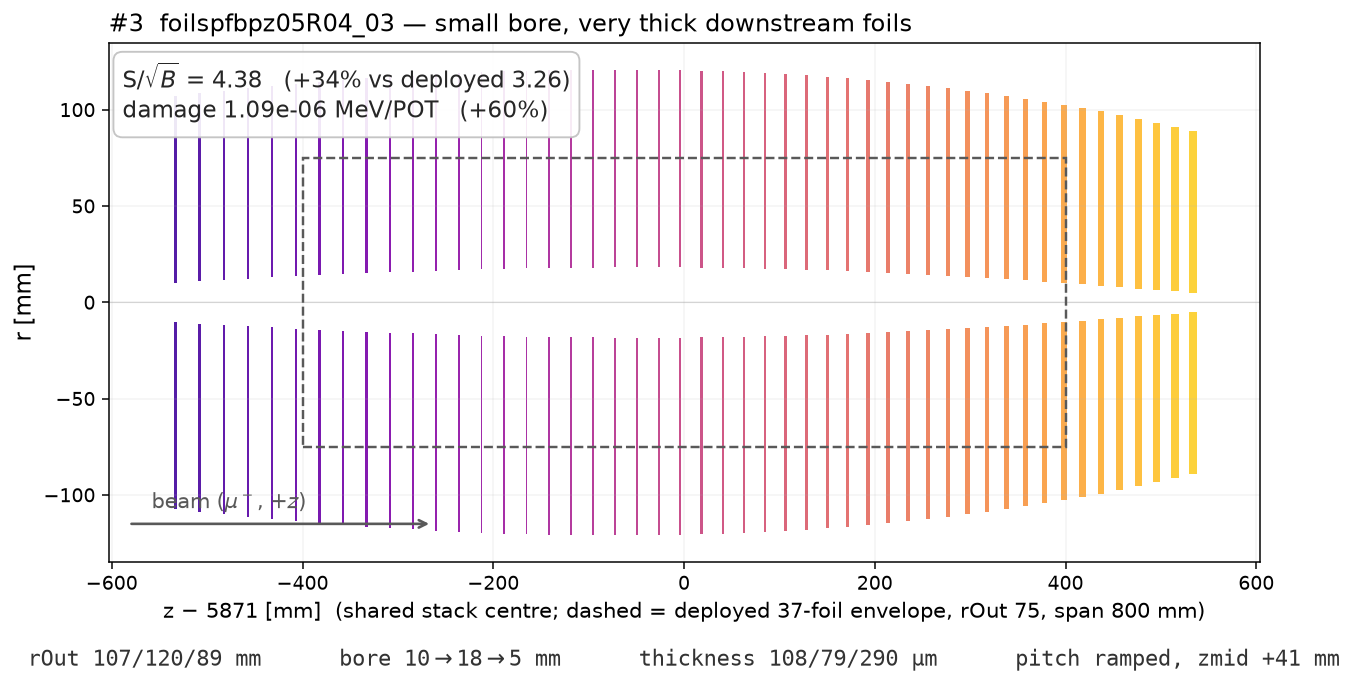
\includegraphics[width=0.95\textwidth]{foilspf_top3_foilspfbpz05R04_03.png}
\end{center}
\end{frame}

\begin{frame}{\#4 --- \texttt{bpz05R08\_00}, S/$\sqrt{B}$ = 4.38}
\begin{center}
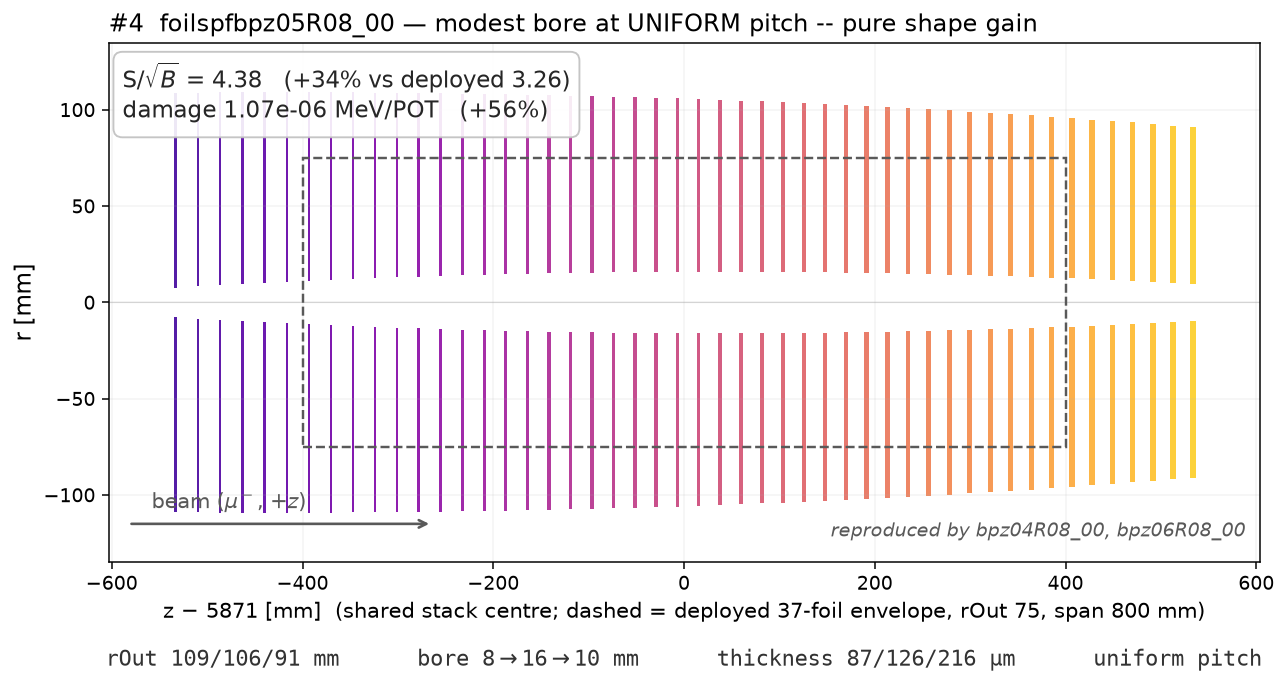
\includegraphics[width=0.95\textwidth]{foilspf_top4_foilspfbpz05R08_00.png}
\end{center}
\end{frame}

\begin{frame}{\#5 --- \texttt{bpz06R11\_00}, S/$\sqrt{B}$ = 4.38}
\begin{center}
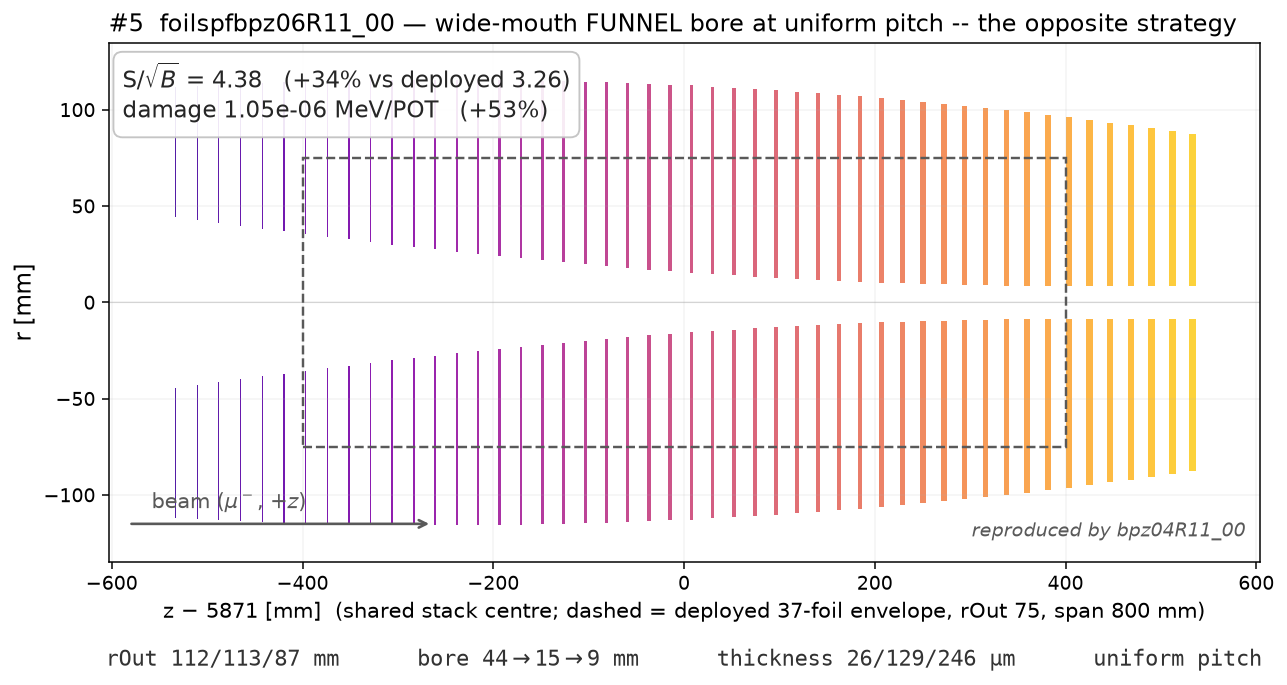
\includegraphics[width=0.95\textwidth]{foilspf_top5_foilspfbpz06R11_00.png}
\end{center}
\end{frame}

% ------------------------------------------------- what BO actually is
\begin{frame}{What ``GP surrogate $+$ multi-objective acquisition'' means}
\small
\textbf{GP surrogate --- the map.}
Each real evaluation costs $\sim$150 CPU-hours, so we cannot try many designs. The Gaussian
Process looks at every design tried so far and draws a map of the whole space: for a design we
have \emph{not} tried it predicts the answer \textbf{and how unsure it is}. Near measured points
the prediction is sharp; far away it is foggy. \emph{The fog is the useful part.}
\vspace{0.7em}

\textbf{Acquisition --- the rule for where to go next.}
Something has to choose which 10 designs to actually simulate next. The acquisition function
trades off \textbf{exploit} (go where the map predicts good results) against \textbf{explore}
(go where the fog is thick --- we might be missing something).
\vspace{0.7em}

\textbf{Multi-objective --- why there is no single ``best''.}
We want two things at once: more signal, less detector damage. They fight each other, so there
is no single winner --- there is a \textbf{set} of best compromises, the \textbf{Pareto front}
(the map on the status slide). Our acquisition function (\texttt{qNEHVI}) picks the designs
expected to push that frontier \emph{outward} the most, rather than chasing one number.
\end{frame}

\end{document}
